\section{螺母}
\begin{procedure}
\item 切换视图方向

首先将视图方向切换为西南等轴测。

\begin{lstlisting}
命令: -VIEW
输入选项 [?/删除(D)/正交(O)/恢复(R)/保存(S)/设置(E)/窗口(W)]: swiso
\end{lstlisting}

再将用户坐标系的$xy$平面切换为与主视图平行。

\begin{lstlisting}
命令: UCS
当前 UCS 名称: *世界*
指定 UCS 的原点或 [面(F)/命名(NA)/对象(OB)/上一个(P)/视图(V)/世界(W)/X/Y/Z/Z 轴(ZA)] <世界>: za
指定新原点或 [对象(O)] <0,0,0>:
在正 Z 轴范围上指定点 <0.0000,0.0000,1.0000>: 0,1,0
\end{lstlisting}

\item 构建正六面体

忽略螺母零件中的倒角边和孔后,主视图投影仅剩下一正六边形。根据正方体的投影经验,可知其表达的是一个正六面体,也称正六棱柱。图\ref{fig:sixnenzhu}为正六棱柱的立体图,图\ref{fig:sixnenthreeview}为正六棱柱的投影视图,从视图中可以看出,其顶面与底面的水平面投影重合并映实形,为一正六边形;六个棱面在水平投影面积聚为正六边形的六条边。

\begin{figure}[htbp]
\centering
\subfloat[]{\label{fig:sixnenzhu}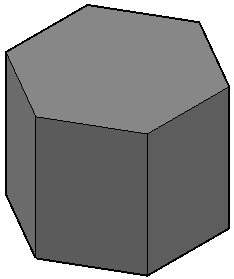
\includegraphics[scale=0.7]{sixnenzhu.png}}\hspace{30pt}
\subfloat[]{\label{fig:sixnenthreeview}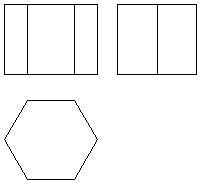
\includegraphics[scale=1]{sixnenthreeview.png}}
\caption{正六棱柱的投影}
\end{figure}

在AutoCAD中构建六棱柱实体需要用到棱锥体命令,其调用方法有:
\begin{itemize}
\item 键盘输入PYRAMID\index{pyramid,棱锥体}或pyr
\item 【绘图】$\rightarrow $【建模】$\rightarrow $【棱锥体】
\item 【实体】
\includegraphics[scale=0.45]{solidtoolbar}工具栏中的【棱锥体】
\includegraphics[scale=0.5]{pyramidtool}图标
\end{itemize}

调用棱锥体命令后,命令提示当前的侧面数为4。由于螺母的主视图是六边形,因此其侧面数6个,故需要选择【侧面(s)】选项将侧面数修改为6个。

\begin{lstlisting}
命令: PYRAMID
 4 个侧面  外切
指定底面的中心点或 [边(E)/侧面(S)]: s
输入侧面数 <4>: 6
\end{lstlisting}

完成侧面数的修改后,在AutoCAD的绘图区域任意指定一点做为底面的中心,并指定底面半径为12.5。此时在绘图区显示绘制的是棱锥体,如图\ref{fig:taihuluomu1} 所示,

\begin{figure}[htbp]
\centering
\subfloat[]{\label{fig:taihuluomu1}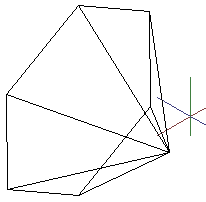
\includegraphics[width=0.4\textwidth]{taihuluomu1}}\hspace{20pt}
\subfloat[]{\label{fig:taihuluomu2}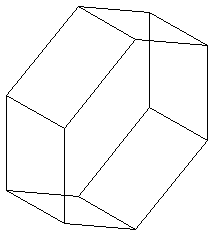
\includegraphics[width=0.4\textwidth]{taihuluomu2}}
\caption{构建正六棱柱}
\end{figure}

\begin{lstlisting}
指定底面的中心点或 [边(E)/侧面(S)]:
指定底面半径或 [内接(I)]: 12.5
\end{lstlisting}

由于AutoCAD的棱锥体命令默认是绘制棱锥体。棱锥体可以看作顶面半径为零的直棱体,因此需要使用【顶面半径(T)】选项修改顶面半径为12.5。

\begin{lstlisting}
指定高度或 [两点(2P)/轴端点(A)/顶面半径(T)]: t
指定顶面半径 <0.0000>: 12.5
\end{lstlisting}

最后指定六棱柱的高度为10,结果如图\ref{fig:taihuluomu2}所示。

\begin{lstlisting}
指定高度或 [两点(2P)/轴端点(A)]: 10
\end{lstlisting}

\item 构建螺母基础孔

为方便螺母基础孔的定位,我们在正六棱柱上绘制一条图 所示的辅助线。

\begin{figure}[htbp]
\centering
\subfloat[]{\label{fig:taihuluomu3}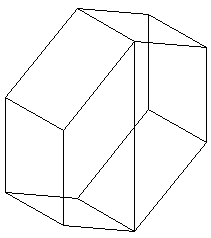
\includegraphics[width=0.4\textwidth]{taihuluomu3}}\hspace{20pt}
\subfloat[]{\label{fig:taihuluomu4}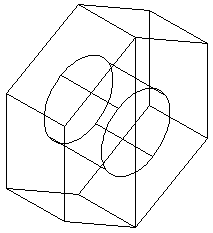
\includegraphics[width=0.4\textwidth]{taihuluomu4}}
\caption{构建基础孔}
\end{figure}

\begin{lstlisting}
命令: line
指定第一个点:
指定下一点或 [放弃(U)]:
指定下一点或 [放弃(U)]:
\end{lstlisting}


然后以辅助组的中点做为基础孔圆柱体的底面圆心,绘制基础孔圆柱体。

\begin{lstlisting}
命令: CYLINDER
指定底面的中心点或 [三点(3P)/两点(2P)/切点、切点、半径(T)/椭圆(E)]:
指定底面半径或 [直径(D)] <14.4338>: 6
指定高度或 [两点(2P)/轴端点(A)] <10.0000>:10
\end{lstlisting}

最后从正六棱体中去除基础孔圆柱。

\begin{lstlisting}
命令: SUBTRACT
选择要从中减去的实体、曲面和面域...
选择对象: 找到 1 个
选择对象:  选择要减去的实体、曲面和面域...
选择对象: 找到 1 个
选择对象:
\end{lstlisting}

\item 构建螺母倒角边

 \begin{figure}[htbp]
 \centering
\subfloat[]{\label{fig:jiejiao1}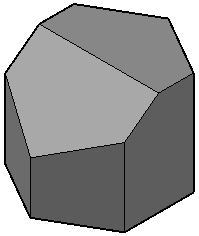
\includegraphics[scale=0.8]{jiejiao1.png}}\hspace{30pt}
\subfloat[]{\label{fig:jiejiao2}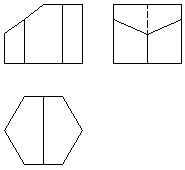
\includegraphics[scale=1]{jiejiao2.png}}
\caption{正六棱柱的截交线}
\end{figure}

通过观察螺母的视图表示,可以看出螺母的倒角边比较特别,仅仅倒去棱线所在的角。为什么会作出如此判断呢?首先,让我们来了解一下截交线的概念。所谓截交线是指一个或多个平面切割立体所产生的表面交线。用于切割立体的平面既可是平面也可以是曲面。图\ref{fig:jiejiao1}为一个倾斜于正六棱柱轴线且过顶面的截面切割的结果,其截面为五边形封闭线框。由图\ref{fig:jiejiao2}所示的三视图可知,该封闭线框构成的平面区域垂直于$V$投影面,投影为一积聚直线,其俯视图和左视图投影为类似形的封闭五边形。

根据平面截交正六棱柱的截交线特点和螺母倒角边的视图细节,可以推断出其截交平面是一圆锥曲面。在AutoCAD中是无法用倒角边命令直接实现这样的倒角边建模的。因此需要先以辅助线的中点作为圆柱体的底面中心,构建半径为12.5的辅助圆柱体,结果如图\ref{fig:taihuluomu5} 所示。

\begin{figure}[htbp]
\centering
\subfloat[]{\label{fig:taihuluomu5}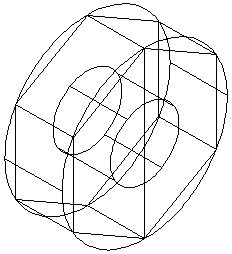
\includegraphics[width=0.4\textwidth]{taihuluomu5}}\hspace{20pt}
\subfloat[]{\label{fig:taihuluomu6}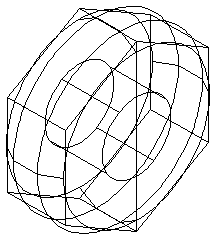
\includegraphics[width=0.4\textwidth]{taihuluomu6}}
\caption{构建辅助圆柱}
\end{figure}

\begin{lstlisting}
命令: CYLINDER
指定底面的中心点或 [三点(3P)/两点(2P)/切点、切点、半径(T)/椭圆(E)]:
指定底面半径或 [直径(D)] <6.0000>: 12.5
指定高度或 [两点(2P)/轴端点(A)] <10.0000>:
\end{lstlisting}

构建完辅助圆柱体后,根据螺母的尺寸应用【表达式(E)】选项来完成圆柱体上倒角边的距离尺寸计算。倒角边结果如图\ref{fig:taihuluomu6}所示。

\begin{lstlisting}
命令: CHAMFEREDGE
距离 1 = 1.0000,距离 2 = 1.0000
选择一条边或 [环(L)/距离(D)]: d
指定距离 1 或 [表达式(E)] <1.0000>: e
输入表达式:(12.5-12.5*cos(30))*tan(60) 
指定距离 2 或 [表达式(E)] <1.0000>: e
输入表达式: 12.5-12.5*cos(30)
选择一条边或 [环(L)/距离(D)]:
选择同一个面上的其他边或 [环(L)/距离(D)]:
选择同一个面上的其他边或 [环(L)/距离(D)]:
按 Enter 键接受倒角或 [距离(D)]:
\end{lstlisting}

由于整个正六棱柱内接于所构建的辅助圆柱体,因此这两实体除孔和棱角处没有交集外,其余均是公共的。因此应该用集合中的交集来构建两个实体之间的公共部分。在AutoCAD中调用交集命令的方法有:
\begin{itemize}
\item 键盘输入intersect\index{intersect,交集}或in
\item 【修改】$\rightarrow $【实体编辑】$\rightarrow $【交集】
\item 【实体编辑】
\includegraphics[scale=0.45]{solidedittools}工具栏中的【交集】
\includegraphics[scale=0.5]{intersecttool}图标
\end{itemize}

交集命令调用后,选择正六棱柱和辅助圆柱体作为求交集对象,选择后的效果如图 所示。

\begin{figure}[htbp]
\centering
\subfloat[]{\label{fig:taihuluomu7}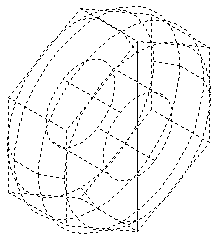
\includegraphics[width=0.4\textwidth]{taihuluomu7}}\hspace{20pt}
\subfloat[]{\label{fig:taihuluomu8}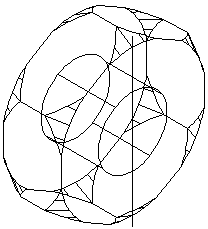
\includegraphics[width=0.4\textwidth]{taihuluomu8}}
\caption{交集操作过程}
\end{figure}

\begin{lstlisting}
命令: INTERSECT
选择对象: 找到 1 个
选择对象: 找到 1 个,总计 2 个
选择对象:
\end{lstlisting}

\item 删除辅助线

接下来删除模型中的辅助线,完成后结果如图所示。
\begin{lstlisting}
命令: erase
选择对象: 找到 1 个
选择对象:
\end{lstlisting}

\item 切换视觉样式

为便于观察,最后将模型的视觉样式切换为灰度样式,模型结果如图所示。


\begin{lstlisting}
命令: vscurrent
输入选项 [二维线框(2)/线框(W)/隐藏(H)/真实(R)/概念(C)/着色(S)/带边缘着色(E)/灰度(G)/勾画(SK)/X 射线(X)/其他(O)] <二维线框>: g
\end{lstlisting}

\begin{figure}[htbp]
\centering
\begin{floatrow}[2]
\ffigbox{\caption{删除辅助线}\label{fig:taihuluomu9}}{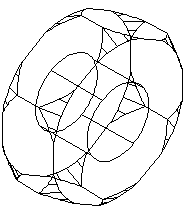
\includegraphics[width=0.4\textwidth]{taihuluomu9}}
\ffigbox{\caption{螺母模型}\label{fig:taihuluomu10}}{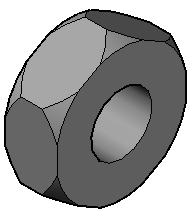
\includegraphics[width=0.4\textwidth]{taihuluomu10}}
\end{floatrow}
\end{figure}
\item 保存模型

最后,将模型以文件名“螺母.dwg”进行保存。
\end{procedure}
\endinput